\chapter{はじめに}

\section{研究の背景}
当研究室では,毎年NHK高専ロボットコンテストに参加するためのロボット設計,及び製作を行っ
ている.過去三年間全国大会に出場しており,本校の名称が金沢工業高等専門学校である最後の年で
もあり今年度は地区大会での優勝を目標にしてて取り組んだ.

私たちは,目標達成のためには高速な移動ができるロボットが必要だと考え,ロボットの移動
方法をタイヤの二輪駆動に決め,使用するDCモータに高出力なものを使用した.
そのため,30Aでも問題ない高出力モータドライバが必要だった.そこで,伊藤研究室で
昨年作成されたITOLAB MOTORDRIVERを使用した.しかし,多くの不具合が発生したので問題解決
に向けて対策をとったものの,目標とした移動速度を下回った状態で大会に挑むこととなった.

地区大会では,初戦に一台のロボットの移動操作ができなくなるマシントラブルに遭い,地区大会
一回戦敗退という無念な結果となった.

その後,マシントラブルはモータドライバに異常があったのではという話になったが,原因を見
つけることはできなかった.
今年度のNHK高専ロボットコンテストの結果から,来年の当研究室のロボットが活躍するために,
扱いやすい高出力モータードライバが有効だと考える.

今年度のNHK高専ロボットコンテストロボットと,ロボットの足回りのモータを図\ref{fig:hontai}
と図\ref{fig:motoru}に示す.
\begin{figure}[H]
  \begin{center}
    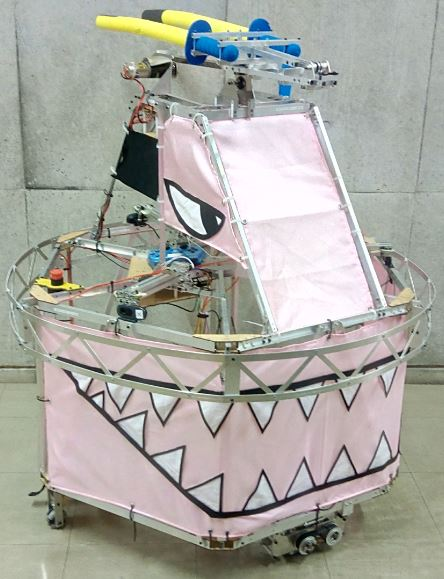
\includegraphics[width=150mm]{hontai}
    \end{center}
  \caption{ロボコンロボット}
 \label{fig:hontai}
\end{figure}
\begin{figure}[H]
  \begin{center}
    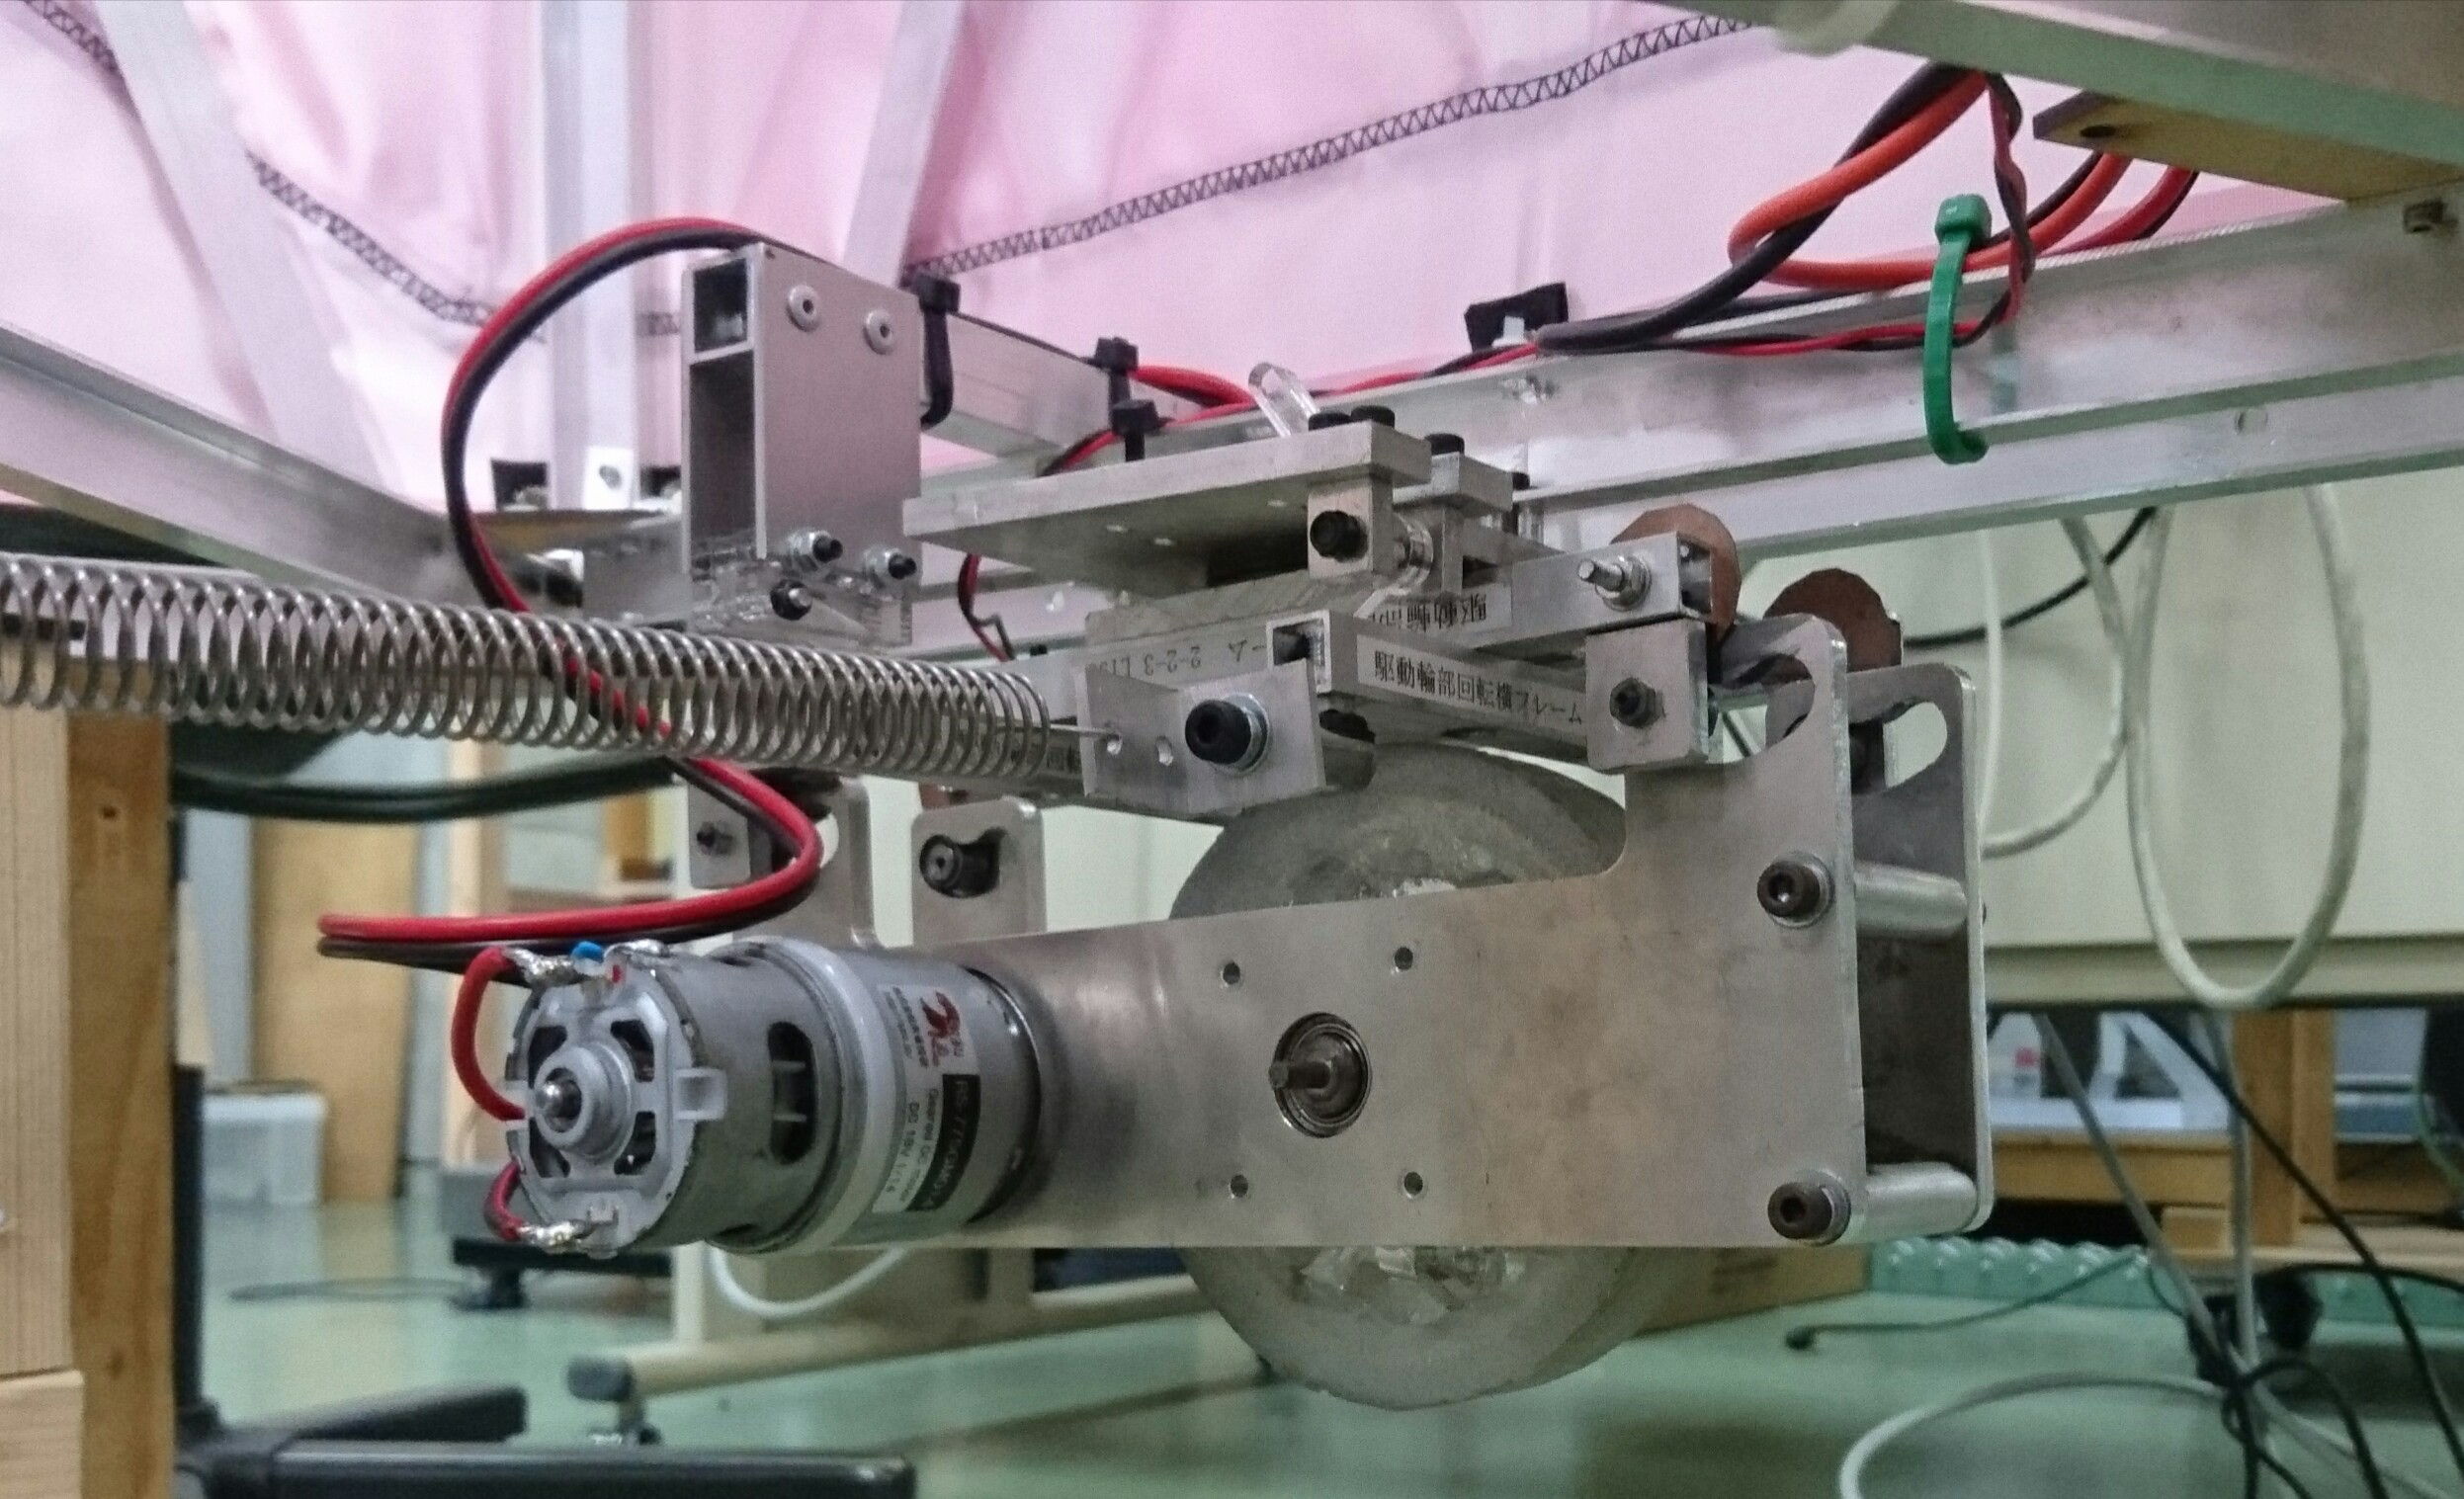
\includegraphics[width=150mm]{motoru}
    \end{center}
  \caption{足回りのモータ}
 \label{fig:motoru}
\end{figure}

\section{研究の目的}
ITOLAB MOTORDRIVERを基に,当研究室で使用できる高出力モータードライバの設計,製作を行う.

\section{本論文の構成}
1章では,本研究の背景と簡略化した概要を示す.2章では,今年のロボコンで使用した
ITOLAB MOTORDRIVERについて述べる.3章では,今回の研究で作成した高出力
モータドライバについて述べる.4章で,最後に本研究のまとめを述べる.